\documentclass[oneside]{ausarbeitung}
\bibliography{latexlit}

\usepackage{float}
\usepackage{url}

% ----------------------------------------------------------------------

\begin{document}

%--- Sprachauswahl
% Erlaubte Werte:
%   \selectlanguage{english}
%   \selectlanguage{ngerman}
\selectlanguage{ngerman}

%--- Art der Arbeit
% Erlaubte Werte:
%   \Praxissemesterbericht
%   \Projektbericht
%   \Bachelorarbeit
%   \Seminararbeit
%   \Masterarbeit

\Projektbericht

%--- Studiengang:
% Erlaubte Werte:
%   \Informatik
%   \Elektronik
%   \DataScience
\Informatik

\title{Algorithmisches Handeln von Kryptowährungen}

\author{Sebastian Flum}
\matrikelnr{76855}

%--- Ist der Erstbetreuer (\examinerA) an der Hochschule ein Professor?
% Erlaubte Werte:
%   \examinerIsAProfessortrue   % Ja
%   \examinerIsAProfessorfalse  % Nein
\examinerIsAProfessorfalse

%--- Betreuer
\examinerA{Sebastian Stigler}
%\examinerB{Prof.~Dr.~Ulrich~Klauck}

%--- Einreichungsdatum
\date{28. Februar 2021}

%--- Titelseite Anzeigen
\maketitle
\cleardoublepage

%---
\pagenumbering{roman}
\setcounter{page}{1}

%--- Eidesstattliche Erklärung anzeigen
\makeaffirmation
\cleardoublepage

%---------------------------------------------------
\begin{abstract}
\label{abstract}

Beim algorithmischen Handeln werden Handelsentscheidungen auf der
Grundlage zuvor definierter Anweisungen und Regeln getroffen, die in
Form eines Computerprogramms umgesetzt wurden. Dabei wird Code
geschrieben, der die Trades im Namen des Händlers oder Investors
ausführt, wenn bestimmte Bedingungen erfüllt sind.  

Im Rahmen dieser Arbeit wurde versucht, jenes Verfahren auf den Handel
von kryptographischen Währungen wie Bitcoin oder Ethereum anzuwenden
und den Grundstein eines algorithmisches Handelssystem für diese zu
entwerfen. So soll herausgefunden werden, ob der automatisierte Handel
von Kryptowährungen, durch ein selbst entwickeltes System,
erfolgreich sein kann.

Dabei beschäftigt sich diese Arbeit im grundlegenden mit folgenden Konzepten:

\begin{enumerate}
	\item Algorithmische Handelsstrategien und technische Indikatoren
	\item Implementierung einer Schnittstelle für Handelsplattformen
	\item Backtesting von Handelsstrategien
	\item Entwurf und Verwaltung eines Trading Bots
	\item Erstellung einer Konsolenanwendung
	\item Verknüpfung dieser Elemente innerhalb eines modularen Systems
\end{enumerate}

Umgesetzt wurde dieses Projekt fast ausschließlich unter der
objektorientierten Verwendung der Programmiersprache Python, in
Verbindung mit einigen wenigen HTML Elementen.

\end{abstract}

%---------------------------------------------------
\cleardoublepage
\tableofcontents

%---
\listoffigures

%---
\listoftables

%---
\listoflistings

%---
\listofabbreviations
\begin{acronym}[API]  % Längstes Kürzel in der nachfolgenden
                       % Liste um die Breite der Spalte für die
                       % Abkürzungen zu bestimmen.

%% Eintrag: \acro{Referenzname}[Kürzel]{Langform}
%% Im Text wird die Abkürzung dann mit \ac{Referenzname} benutzt.
\acro{api}[API]{Application Programming Interface}
\acro{sma}[SMA]{Simple Moving Average}
\acro{cfd}[CFD]{Contract for Difference}
\acro{rest}[REST]{Representational State Transfer}
\acro{http}[HTTP]{Hypertext Transfer Protocol}
\acro{pandas}[Pandas]{Python Data Analysis Library}
\acro{url}[URL]{Uniform Resource Locator} 
\end{acronym}
%---


\cleardoublepage
\pagenumbering{arabic}
\setcounter{page}{1}

%---------------------------------------------------
\chapter{Einleitung}
\label{cha:einleitung}

"Neues Allzeithoch: Bitcoin-Rekordjagd geht ungebremst
weiter"\cite{bitcoin_artikel_1}. "Kryptowährung: Bitcoin knackt Marke
von 50.000 Dollar"\cite{bitcoin_artikel_2}. Artikel wie diese sind
schon lange keine Seltenheit mehr. Kryptowährungen, allen voran der
Bitcoin, entwickelten sich in den letzten Jahren zum Sinnbild
schnellen Reichtums. Doch das war nicht immer so. Im Jahre 2011, als
sich der Bitcoin noch in seinen Kinderschuhen befand, kostete ein Coin
gerade einmal 1 Dollar\cite{bitcoin_kurs_2011}. Vielleicht erwischt
man sich nun selbst bei dem Gedanken daran, was wohl wäre, wenn man
zu dieser Zeit schon das Potential dieser, damals unscheinbaren,
Internetwährung erkannt hätte. Einige vorausdenkende Köpfe
erkannten dies frühzeitig und wurden dadurch reich. Andere wiederum
nutzten die neu entdeckte Kryptowährung dazu, online für ihre Pizza
zu bezahlen. Verrückt, wenn man sich vor Augen führt, dass man mit
der selben Menge Bitcoins heute zehntausende Pizzen bezahlen könnte.
Vielleicht lässt dieser Gedanke die Herzen einiger Pizzaliebhaber
höher schlagen, vorrangig stellt sich jedoch die Frage, ob man mit
dem Besitz und Handel von Kryptowährungen heutzutage noch Erfolg
haben kann. Und wenn ja - kann das auch ein Computerprogramm?


\section{Motivation}
\label{sec:motivation}

Natürlich stellt die Aussicht auf realisierbaren Gewinn, erzeugt
durch ein selbst entwickeltes Handelssystem, ein großer
Motivationsfaktor dar - doch es ist mehr als das. Kryptowährungen
liegen einem faszinierendem Stück Technologie zugrunde. Der
sogenannten \textbf{Blockchain} (dazu später mehr). Dennoch können
die digitalen Währungen wie jede herkömmliche Währung getauscht und
gehandelt werden, befinden sich gleichzeitig aber außerhalb der
Kontrolle finanzieller Institutionen. Somit verbinden Kryptowährungen
die Welt des Finanzhandels mit der Welt der Informatik. Für jemanden,
den der herkömmliche Handel mit Wertpapieren oder Ähnlichem nur
wenig anspricht, bieten Kryptowährungen die Möglichkeit eines
interessanten Einblicks in beide Welten. 

Abgesehen davon finde ich großen Gefallen daran, Lösungen für
gegebene Problemstellungen zu entwerfen und in Programmcode
umzusetzen. Es macht mir Spaß, neue Technologien kennenzulernen und
deren Konzepte praktisch einzusetzen. Der Entwurf eines
algorithmischen Handelssystems bietet dafür die perfekte Grundlage,
da es beliebig erweitert werden kann und viele Schlüsselkonzepte
vereint. So stellt das Projekt eine interessante Möglichkeit für
mich dar, Dinge wie objektorientierte Programmierung, Entwurf von
Softwarearchitekturen und Datenbanken, Web-Entwicklung und vielem
mehr, innerhalb eines zusammenhängenden Projektes, kennenzulernen und
anzuwenden.


\section{Problemstellung und -abgrenzung}
\label{sec:problemstellung}

Als Ganzes betrachtet ist die Problemstellung, ein algorithmisches
Handelssystem zu entwerfen, relativ unüberschaubar. Zur Bewältigung
muss es daher in mehrere Teilprobleme heruntergebrochen werden. Daraus
ergeben sich folgende, im nachfolgenden grob beschriebene,
Problemstellungen:

\textbf{1. Algorithmische Handelsstrategien und technische Indikatoren} \\
Ohne eine geeignete Trading Strategie, die entscheidet, wann Einkäufe
und Verkäufe zu tätigen sind, kann wohl kein System Erfolg haben.
Diesen Trading Strategien liegen technische Indikatoren zu Grunde. Ein
technischer Indikator dient dabei zur alternativen Darstellung der
Kursverläufe und liefert der Strategie wertvolle Analyseinformationen.
Der Fokus soll dabei jedoch weniger auf der Findung und Konzeption
neuer Strategien und Indikatoren liegen, sondern darauf, wie diese
möglichst einfach und modular in das System eingebunden werden
können.

\textbf{2. Entwurf einer Schnittstelle für Handelsplattformen} \\
Der Handel von Kryptowährungen mittels eines algorithmischen Systems
erfordert, genauso wie beim Handeln von Hand, eine Plattform, auf der
die Ein- und Verkäufe getätigt werden. Im Vergleich zum Handeln von
Hand, benötigt das Trading-System jedoch ein \ac{api}, an die es
anknüpfen kann, um mögliche Aktionen der Plattform tätigen zu
können. Einige Plattformen bieten solche APIs zum Teil kostenlos an.
Die Problemstellung ergibt sich daraus, die von den Plattformen
bereitgestellten APIs zu nutzen und eigene, möglichst modulare,
Schnittstellen zur Verwendung dieser zu entwerfen.

\textbf{3. Backtesting von Handelsstrategien} \\
Backtesting bzw. Rückvergleich bezeichnet den Prozess, eine Strategie
zu evaluieren, indem die Strategie auf historische Daten angewandt
wird\cite{backtesting_definition}. Findet man beispielsweise eine neue,
vielversprechende Trading
Strategie und möchte diese nun nach der Umsetzung in Code testen, ist
es sehr riskant, die Strategie im Echtzeitbetrieb laufen zu lassen.
Sollte die Strategie nämlich doch nicht so vielversprechend sein,
läuft man Gefahr, große Verluste durch schlecht platzierte Ein- und
Verkäufe hinnehmen zu müssen. Der Backtest wirkt diesem Risiko
entgegen und stellt somit eine der wichtigsten Komponenten des Systems
dar.

\textbf{4. Entwurf und Verwaltung eines Trading Bots} \\
Echzeitdaten auswerten und automatisiert Einkäufe und Verkäufe
tätigen zu lassen. Da dies den Umfang dieser Arbeit jedoch
übersteigt, soll innerhalb dieses Projekts nur der Grundstein dieses
Features gelegt werden.

\textbf{5. Erstellung einer Konsolenanwendung} \\
Alle Features des zu entwickelnden Systems, sollen dem Nutzer als Teil
einer Konsolenanwendung zur Verfügung stehen. Mit dieser soll es
beispielsweise möglich sein, Backtests sowie neue
"Händler-Instanzen" aka Trading-Bots zu erstellen, welche
verschiedenen Parametern wie Auswahl der Kryptowährung, Strategie,
Kapital, usw. zu Grunde liegen.

\textbf{6. Verknüpfung der Komponenten innerhalb eines modularen Systems} \\
Im laufe der Arbeit werden Lösungskonzepte für die, hier
aufgeführten, Problemstellungen entworfen und implementiert. Wichtig
ist es dabei, die Komponenten mit Hinblick auf das Gesamtsystem und
dessen Erweiterbarkeit/Modularität zu entwerfen, sowie ein sauberes
und klar definiertes Zusammenspiel zu ermöglichen. 

\section{Ziel der Arbeit}
\label{sec:ziel}

Wie sich aus den vorherigen Abschnitten bereits erkennen lässt,
stellt das Ziel dieser Arbeit den Entwurf und die Implementierung
eines algorithmischen Handelssystems für Kryptowährungen dar. Dabei
soll es dem System möglich sein, Marktdaten über Kryptowährungen zu
sammeln und automatisiert auszuwerten. Des weiteren soll das System
über eine Teststrategie sowie den dazugehörigen technischen
Indikatoren enthalten, welche durch einen, ebenfalls im System
implementierten, Backtest ausgewertet werden kann. Dabei soll es dem
System möglich sein, ausgewählte Markdaten und Backtest-Ergebnisse
zu visualisieren und anschaulich darzustellen. Unter anderem soll das
System einen Prototyp eines Trading-Bots enthalten, welcher mit
zukünftigen Erweiterungen in der Lage sein soll, echte
Handelsaktionen durchzuführen. Diese Handelsaktionen werden innerhalb
dieser Arbeit jedoch \underline{nicht} implementiert, d.h. das System
ist innerhalb diesen Projekts nicht in der Lage, eigenständig reale
Käufe und Verkäufe zu tätigten. Die zuvor genannten Funktionen
sollen dem Nutzer letztendlich durch eine Konsolenanwendung
bereitgestellt werden.

\section{Vorgehen}
\label{sec:vorgehen}

Nachdem mit Problemstellung und Ziel gewissermaßen Anfangs- und Endpunkt 
des Praktikums beschrieben sind, wird hier der zur Erreichung des Ziels 
eingeschlagene Weg vorgestellt. Dazu werden typischerweise die folgenden 
Kapitel und ihr Beitrag zur Erreichung des Ziels der Arbeit kurz 
beschrieben. Die folgenden Kapitel sind ein – möglicher – Aufbau, 
Abweichungen können durchaus notwendig sein. Zur Darstellung des 
Vorgehens ist eine grafische Darstellung sinnvoll, bei der die einzelnen 
Lösungsschritte und ihr Zusammenhang dargestellt werden. Ein Beispiel 
hierfür findet sich in Abbildung \ref{fig:1}.

\begin{figure}[htbp]
  \centering
  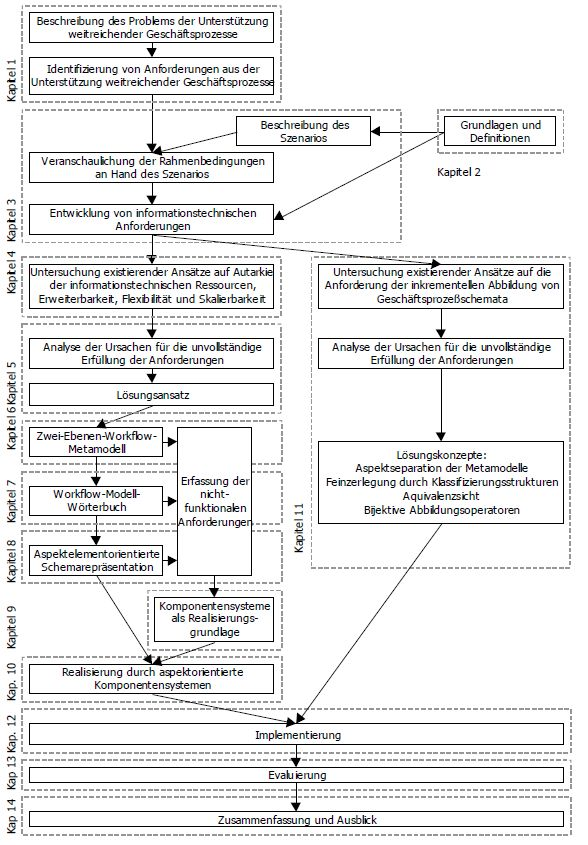
\includegraphics[height=0.9\textheight]{img/ausarbeitung.jpg}
  \caption{vorgehen nach \autocite{Schmidt:Geschaeftsprozesse}}
  \label{fig:1}
\end{figure}

%---------------------------------------------------
\chapter{Grundlagen}
\label{cha:grundlagen}

%----
\section{Trading}
\label{sec:trading}

Das Wort "Trading", zu Deutsch: Handel, stammt aus dem Englischen und
beschreibt den Kauf und Verkauf von Finanzprodukten an einer Börse.
Menschen, die dieser Beschäftigung nachgehen, werden daher auch als
Trader bezeichnet. Ein durchgeführter Handel heißt dementsprechend
also Trade. (vgl. \cite{trading_1})

Trading bedeutet, die Schwankungen der Finanzmärkte mithilfe von
Trades für die eigenen Zwecke zu nutzen. Das heißt kaufen, verkaufen
und dabei Gewinne einstreichen - oder den Verlust verkraften. Durch
das Internet und benutzerfreundliche Trading-Anbieter ist es auch für
Hobby-Anleger möglich, Finanzinstrumente wie Wertpapiere, Währungen,
Rohstoff-Zertifikate oder Ähnlichem zu handeln. Beim Trading handelt
es sich grundsätzlich um Spekulation. Wo ein Trader sein Geld
investiert, ist meist von untergeordneter Wichtigkeit. Beispielsweise
geht es nicht darum, Anteile eines Unternehmens zu kaufen, um
langfristig an dessen Entwicklung teilzuhaben. Das Ziel eines Traders
ist es, durch einen Kursanstieg im Zeitraum des Besitzes eins
Finanzinstruments Gewinn zu erzielen. Das bedeutet, ein Trader kauft
beispielsweise eine Aktie, hofft auf einen Kursanstieg und verkauft
sie dann wieder. Die anschließende Wertdifferenz abzüglich der
Transaktionskosten stellt den Gewinn des Traders dar. (vgl.
\cite{trading_2})

\subsection{Algorithmischer Handel}
\label{sub:algorithmischer_handel}

Algorithmischer beschreibt den automatischen Handel von
Finanzinstrumenten durch Computerprogramme. Dabei folgt das
Computerprogramm einem vordefiniertem Satz von Anweisungen
(Algorithmus), um einen Trade zu platzieren. Die Trades können
theoretisch Gewinne mit einer Geschwindigkeit und Häufigkeit
generieren, die für einen menschlichen Trader unmöglich sind. (vgl.
\cite{algorithmic_trading})

Die definierten Sätze von Anweisungen basieren auf Timing, Preis,
Menge oder einem beliebigen mathematischen Modell. Abgesehen von den
Gewinnmöglichkeiten für den Trader, macht der algorithmische Handel
die Märkte liquider und den Handel systematischer, da der Einfluss
menschlicher Emotionen auf die Handelsaktivität ausgeschlossen wird.
(vgl. \cite{algorithmic_trading})

\subsection{Candlestick Charts}
\label{sub:candlestick_charts}

Ein Candlestick Chart ist ein Finanzdiagramm, mit dem sich die
Kursbewegungen eines Wertpapiers oder Ähnlichem darstellen lassen. Es
besteht aus einer Aneinanderreihung von sogenannten \textbf{Candles}
(Kerzen), welche für die verschiedenste Zeiteinheiten verwendet
werden können und vier zentrale Informationswerte enthalten:

\begin{itemize}
	\item Eröffnungskurs (Open)
	\item Schlusskurs (Close)
	\item Höchstkurs (High)
	\item Tiefstkurs (Low)
\end{itemize}

(vgl. \cite{candlestick_basics})

Die Candles haben gegenüber den früher gängigeren Balkencharts den
Vorteil, optisch anschaulicher zu sein, ohne dabei gleich kompliziert
zu werden. Grundsätzlich wird dabei zwischen zwei verschiedenen
Kerzen unterschieden, welche in der nachfolgenden Abbildung
(Abb. \ref{fig:1}) dargestellt werden. \\

\begin{figure}[H]
  \centering
  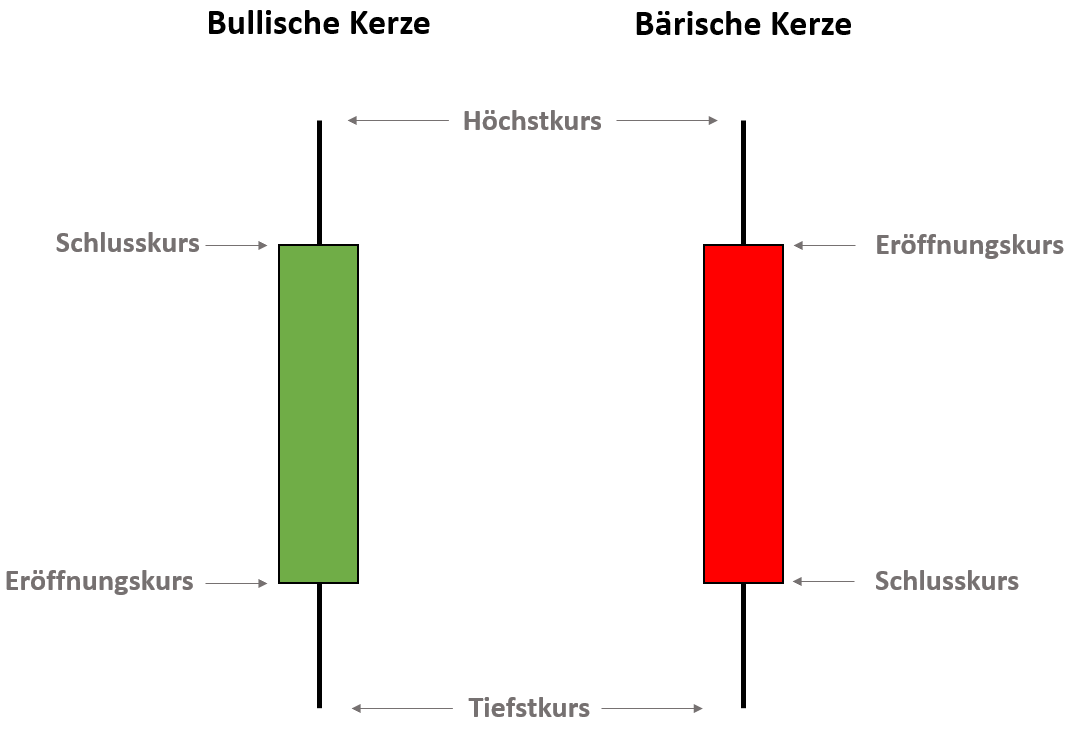
\includegraphics[height=0.45\textheight]{img/candles.png}
  \caption{Kerzen eines Candlestick Charts}
  \label{fig:1}
\end{figure}

Jede Kerze kann dabei für jede beliebige Zeitspanne stehen. Für
einen Tag, eine Woche, einen Monat, oder auch für kurzfristigere
Zeitebenen auf Minutenbasis. Die Aussagen der Kerzen sind dabei jedoch
immer dieselben.

Die Farbe der Candles lässt dabei sofort erkennen, ob es sich um eine
bullische, oder eine bärische Kerze handelt. Die \textbf{bullische
Kerze} symbolisiert ein Zeitintervall, welches positiv verlief, weil
der Schlusskurs über dem Eröffnungskurs des Intervalls lag. Analog
dazu bedeutet die \textbf{bärische Kerze}, dass der Kursverlauf
während des Zeitintervalls der Kerze negativ verlief, weil der
Schlusskurs unter dem Eröffnungskurs lag. Wichtig ist es dabei, sich
im Kopf zu behalten, dass jede Kerze immer nur eine Aussage über den
Kursverlauf ihres Zeitintervalls darstellt. (vgl.
\cite{candles_explained})
 
Fügt man alle Candles zu einem Candlestick Chart zusammen erhält man
ein Diagramm wie in Abbildung \ref{fig:2} dargestellt. \\

\begin{figure}[H]
  \centering
  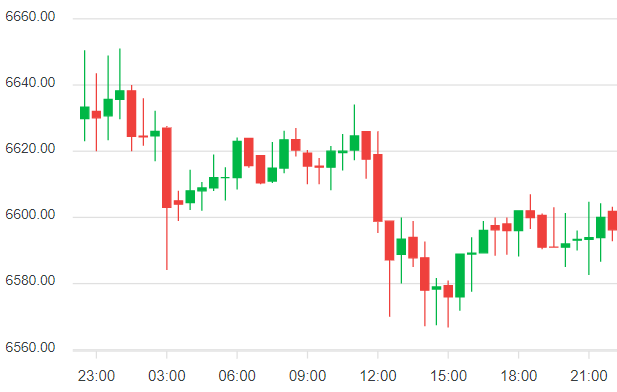
\includegraphics[height=0.43\textheight]{img/candlestick_chart.png}
  \caption{Beispiel eines Candlestick Chart\cite{candlestick_chart_pic}}
  \label{fig:2}
\end{figure}

\subsection{Technische Indikatoren}
\label{sub:technische_Indikatoren}

Technische Indikatoren sind Chart-Analyse-Tools, die Tradern helfen
können, Preisbewegungen besser zu verstehen und darauf zu reagieren.
Es gibt eine riesige Auswahl an technischen Analysewerkzeugen, die
Trends analysieren, Preisdurchschnitte liefern, die Volatilität
(Schwankung) messen und mehr. (vgl. \cite{technical_indicators})

Ein sehr beliebter technischer Indikator ist der \textbf{Moving
Average}, zu Deutsch: gleitender Mittelwert, welcher benutzt wird, um
den durchschnittlichen Schlusskurs des Marktes über einen bestimmten
Zeitraum darzustellen. Trader machen oft Gebrauch von Moving Averages,
da sie ein guter Hinweis auf die aktuelle Marktdynamik sein können.
(vgl. \cite{moving_average})

\textbf{Wie wird ein Moving Average berechnet?} \\
Eine der gängigsten Moving Averages ist der einfache gleitende
Mittelwert bzw. \ac{sma}, welche einfach der Durschnitt aller
Datenpunkte in der Serie geteilt durch die Anzahl der
Punkte\cite{moving_average}.

A = $ \{ $ {a$_{1}$, a$_{2}$, ..., a$_{n}$} $ \} $ \\
n = Number of time periods / price elements

SMA = $\frac{a_1 \ + \ a_2 \ + \ ... \ + \ a_n}{n}$

Betrachtet man zum Beispiel eine 5-Tage-SMA auf einem Tages-Chart von
EUR/USD und die Schlusskurse über die letzten 5 Tage sind wie folgt.

Tag 1: 1.321 \\
Tag 2: 1.301 \\
Tag 3: 1.325 \\
Tag 4: 1.327 \\
Tag 5: 1.326

SMA = (1.321 + 1.301 + 1.325 + 1.327 + 1.326)/5 = 1.32

Veranschaulichen lässt sich dieser Indikator gut in einem Candlestick
Chart, wie in Abbildung \ref{fig:3} dargestellt.

\begin{figure}[H]
  \centering
  \includegraphics[height=0.32\textheight]{img/sma.png}
  \caption{Simple Moving Average (in Gelb) innerhalb eines Candlestick Charts}
  \label{fig:3}
\end{figure} 

\subsection{Trading Strategien}
\label{sub:trading_strategien}

Eine Trading Strategie ist eine Methode zum Kaufen und Verkaufen auf
Märkten, die auf vordefinierten Regeln basiert, die zum Treffen von
Handelsentscheidungen verwendet werden\cite{trading_strategy}.

Es gibt viele Arten von Handelsstrategien, aber sie basieren
größtenteils entweder auf technischen Daten oder auf
Fundamentaldaten. Letzteres beschreibt langfristige, grundlegende
Informationen über die realen Produktionsmöglichkeiten, die
Strukturen der Wirtschaft sowie den Vermögensstatus der
Wirtschaftseinheiten, welche in dieser Arbeit jedoch nicht näher
betrachtet werden\cite{fundamentaldaten}. Die Gemeinsamkeit ist, dass
sich beide auf quantifizierbare Informationen stützen, die auf ihre
Genauigkeit hin rückgetestet werden können.
Technische Handelsstrategien verlassen sich auf technische
Indikatoren, um Handelssignale zu generieren. Technische Trader
glauben, dass alle Informationen über ein bestimmtes Wertpapier o.Ä.
in seinem Preis enthalten sind und dass er sich in Trends bewegt.
(vgl. \cite{trading_strategy}) 

Eine einfache Trading Strategie kann zum Beispiel eine
\textbf{Moving-Average-Strategy} sein, bei welcher ein Kaufsignal
erzeugt wird, sobald der aktuelle Preis einen gewissen Wert unter dem
der Moving Average liegt. Betrachtet man im Hinblick auf diese
Strategie noch einmal Abbildung \ref{fig:3}, lassen sich einige
Stellen im Chart erkennen, bei denen diese Strategie wohl Kaufsignale
erzeugen würde.

\subsection{Order Types}
\label{sub:order_types}

%----

\section{Kryptowährungen}
\label{sec:kryptowährungen}

Eine Kryptowährung ist eine digitale oder virtuelle Währung, die
durch Kryptographie gesichert ist, was es nahezu unmöglich macht, sie
zu fälschen oder doppelt auszugeben. Viele Kryptowährungen sind
dezentralisierte Netzwerke, die auf der Blockchain-Technologie
basieren - einem verteilten Hauptbuch, das von einem verteilten
Netzwerk von Computern erzwungen wird. Ein entscheidendes Merkmal von
Kryptowährungen ist, dass sie im Allgemeinen nicht von einer
zentralen Behörde ausgegeben werden, was sie theoretisch immun gegen
staatliche Eingriffe oder Manipulationen macht.

Die erste Blockchain-basierte Kryptowährung war Bitcoin, die
immernoch die beliebteste und wertvollste ist. Heute gibt es tausende
von alternativen Kryptowährungen mit verschiedenen Funktionen und
Spezifikationen. Einige davon sind Klone oder Abspaltungen von Bicoin,
während andere neue Währungen sind, die von Grund auf neu entwickelt
wurden. (vgl. \cite{cryptocurrency_explained})

\subsection{Die Blockchain}
\label{sub:blockchain}

Trivial ausgedrückt ist eine Blockchain nichts anderes als eine
verteilte, öffentliche Datenbank\cite{blockchain_definition}, wessen
Funktionsprinzip die meisten Kryptowährungen zugrunde
liegen\cite{blockchain_1}.
Um das Prinzip einer Blockchain verstehen zu können, hilft der
Vergleich mit einem Gruppenchat:

Ben, Lisa und Mia haben sich um 14 Uhr im Park verabredet. Diese
Information ist nach dem Absenden auf allen Smartphones im Chatverlauf
gespeichert. Mia überlegt es sich anders und möchte sich erst um 16
Uhr treffen. Diese Entscheidung kann sie aber nicht alleine fällen.
Sie kann auch nicht einfach die Uhrzeit im Chatverlauf nachträglich
ändern. Mia muss also entweder gemeinsam mit den anderen von vorne
planen, oder sie steht um 16 Uhr alleine im Park. Niemand kann
nachträglich etwas verändern. Dieses Prinzip ist der Kern einer
Blockchain, denn auch hier werden Informationen in einem "Verlauf"
gespeichert. Informationen sind hierbei hauptsächlich
Transaktionsinformationen von Nutzern die diese getätigt haben.

Jede Information bildet einen Block, für welche ein Hash -
vergleichbar mit einem digitalen Fingerabdruck - berechnet wird.
Zusätzlich enthält dieser Hash, den Hash des vorherigen Blocks. So
werden die Blöcke über die Hashes, wie in Abbildung \ref{fig:4}
veranschaulicht, zu einer Kette verbunden. Ähnlich wie bei einem
Chatverlauf können die Informationen nicht verändert werden.
Verändert sich nämlich die Information, verändert sich auch der
Hash und die Kette würde auseinander brechen. Genau wie Mia und ihre
Freunde mit der Planung von vorne beginnen müssten, müssten die
Hashes aller folgenden Blöcke neu berechnet werden. (vgl.
\cite{blockchain})

\begin{figure}[H]
  \centering
  \includegraphics[height=0.16\textheight]{img/blockchain.png}
  \caption{Veranschaulichung einer Blockchain\cite{blockchain}}
  \label{fig:4}
\end{figure} 

Die Blockchain wird über ein dezentrales Netzwerk verwaltet, dem
jeder beitreten kann. Jedes Mitglied hat eine vollständige Kopie der
kompletten Blockchain auf dem Computer, welche von diesem auch
geprüft wird. Ein neuer Block wird erst hinzugefügt, wenn ihn jeder
im Netzwerk verifiziert hat. Jeder kontrolliert sozusagen jeden, was
die Blockchain damit sehr sicher macht. Wichtig ist dabei aber nicht
der Mensch vor dem Computer, oder eine dritte Instanz wie
beispielsweise ein Notar. Die Kontrolle, und somit das Vertrauen,
werden von der Blockchain technisch hergestellt. (vgl.
\cite{blockchain})

\subsection{Mining}
\label{sub:mining}

Wie das Geld herkömmlicher Währungen wie beispielsweise Euro oder
Dollar entsteht, ist kein Geheimnis. Das Bargeld entsteht unter
staatlicher Regie. Das Recht zur Prägung von Münzen liegt direkt
beim Staat, während die staatliche Bundesbank Scheine herstellt.
Beides müssen die privaten Geschäftsbanken bei der Bundesbank
kaufen. (vgl. \cite{herstellung_fiat_waehrung}). Doch wie funktioniert
dies bei Kryptowährungen?  

Instanzen einer Kryptowährung werden bei einem Prozess erzeugt, der
\textbf{Mining}, zu Deutsch: Bergbau, genannt wird. Diese Analogie ist
eigentlich recht passend, da neue Coins nur gefunden werden können,
wenn ein bestimmter Arbeitsaufwand betrieben wird.

Der vorrangige Sinn des Minings ist jedoch nicht die Erschaffung von
Coins, welcher eher als Nebeneffekt zu verstehen ist. Der Sinn des
Mining ist vor allem das Verifizieren und Durchführen von
Transaktionen sowie die Überprüfung, ob sich alle Teilnehmer des
Netzwerks an dessen Regeln halten. Der Prozess des Minings wird dabei
von Minern - also Computern mit Rechenleistung - durchgeführt. Wie
bereits in Unterkapitel \ref{sub:blockchain} beschrieben, enthalten
die Blöcke gewisse Transaktionsinformationen. Zustäzlich zu diesen
Transaktionsinformationen besitzt jeder Block eine \textbf{Coinbase
Transaktion}, welche neue Coins enthält, die dann als "Belohnung"
für das Sichern des Netzwerkes an die Miner ausgezahlt werden.  

Ein Miner versucht im Endeffekt also, Transaktionen zu einem Block zu
verbinden. Hat er diese Transaktionsinformationen zu einem passenden
Block verbunden, wird er der Blockchain hinzugefügt und der Miner
für seine Arbeistleistung bezahlt. Veranschaulichen lässt sich
dieser Prozess durch die Analogie eines Puzzles.  Hierbei versucht der
Miner, das Bild des Puzzles (Blockchain) zu bilden, indem er
Puzzlestücke (Blöcke) zusammenfügt. Wer das passende Puzzlestück
findet, erhält die Belohnung. (vgl. \cite{mining})


\subsection{Handel von Kryptowährungen}
\label{sub:handel_von_kryptowährungen}

Kryptowährungen werden in sogenannten \textbf{Wallets} gespeichert.
Das sind digitale Geldbörsen, die auf den unterschiedlichsten
digitalen Geräten wie beispielsweise einem Computer, Smartphone oder
USB-Stick liegen können. Anders als beim klassischen Geldsystem, wo
das Geld bei einer Bank und innerhalb eines Girokontos verwaltet wird,
gehören diese Wallets nur dem Besitzer, was bedeutet, dass niemand
diese Geldbörsen sperren kann. Auch viele andere Einschränkungen
normaler Wärhungen kennt eine Kryptowährung nicht. So gibt es
beispielsweise keine Überweisungslimits, maximale Transaktionshöhen
oder geografische Einschränkungen. Überweisungen können problemlos
von jedem Ort der Welt an jeden Ort der Welt gesendet werden, solange
Sender und Empfänger Internetzugang haben und ein Wallet besitzen.
(vgl. \cite{bitcoins_erklärung})

Wer sich nun dazu entschlossen hat mit Kryptowährungen zu handeln,
hat generell zwei Möglichkeiten:

\textbf{1. Bitcoins kaufen} \\
Der direkte Weg wäre Coins zu kaufen und diese solange zu halten, bis
der erwünschte Kursanstieg erreicht wurde, um sie dann wieder zu
verkaufen. Dazu wird jedoch, wie oben beschrieben, ein Wallet
benötigt. Die Coins werden dann auf Exchange Börsen oder
Krypto-Marktplätzen im Internet gekauft und an das eigene Wallet
geschickt.  

\textbf{2. Trading über CFDs} \\
Alternativ besteht die Möglichkeit des Crypto Trading per \ac{cfd}.
Hierbei spekulieren Anleger lediglich auf den Anstieg bzw. den Fall
des Bitcoin Kurses. Dabei können Basiswerte festegelegt werden, zu
denen die CFDs gekauft bzw. verkauft werden sollen. Steigt der Bitcoin
im Wert um 10\%, dann steigt auch der Wert der erworbenen CFDs um
10\%. (vgl. \cite{crypto_trading})

%----

\section{Application Programming Interface}
\label{sec:api}

Ein Application Programming Interface, bzw. Programmierschnittstelle,
ist ein Programmteil, der von einem Softwaresystem anderen Programmen
zur Anbindung an das System zur Verfügung gestellt wird. Die
Programmanbindung findet dabei auf Quelltext-Ebene statt. (vgl.
\cite{api_definition})

Ein Restaurant bildet ein System. Kunden wollen dieses System nutzen,
indem sie mithilfe einer Essenskarte Bestellungen aufgeben. Dabei ist
die Küche der Teil des Systems, der die Bestellungen der Gäste
zubereitet. Was fehlt, ist das entscheidende Bindeglied, um die
Bestellung der Kunden an die Küche zu übermitteln und ihnen ihr
Essen an den Tisch zu liefern. An dieser Stelle kommt der Kellner ins
Spiel. Der Kellner ist der Bote, bzw. \ac{api}, der die Anfrage der
Kunden entgegennimmt und der Küche - bzw. dem System - mitteilt, was
zu tun ist. Dann liefert der Kellner die Antwort an den Kunden
zurück. In diesem Fall ist es das Essen. (vgl. \cite{api_example})    

\subsection{REST API}
\label{sub:rest_api}
REST steht für Representational State Transfer und beschreibt ein
Paradigma (grunsätzliche Denkweise) für die Softwarearchitektur von
verteilten Systemen, insbesondere für Webservices. \ac{rest} ist eine
Abstraktion der Struktur und des Verhaltens des World Wide Web und hat
das Ziel, einen Architekturstil zu schaffen, der die Anforderungen des
moderen Web besser darstellt. Der Zweck von \ac{rest} liegt
schwerpunktmäßig auf der Kommunikation zwischen Client und Server in
Netzwerken. Eine \ac{rest} \ac{api} ist demnach also eine
Programmierschnittstelle die diesem Paradigma folgt. (vgl.
\cite{rest})

Die Funktionsweise wird in Abbildung \ref{fig:5} ersichtlich.

\begin{figure}[H]
  \centering
  \includegraphics[height=0.35\textheight]{img/rest_api.jpeg}
  \caption{Funktionsweise einer REST API\cite{rest_pic}}
  \label{fig:5}
\end{figure}

Die \ac{api} kommuniziert mit dem Server über das sogenannte
\ac{http} - ein Protokoll zur Übertragung von Daten über ein
Rechnernetz. Es wird hauptsächlich eingesetzt, um Websiten aus dem
World Wide Web in einen Webbrowser zu laden\cite{http_definition}.
Mittels \ac{http} Request, werden also Informationen vom Server
angefordert, wodurch der Server wiederum eine \ac{http} Response
erzeugt, die der Client dann erhält. Um eine Request an die
\ac{api} zu senden, werden \ac{url} benutzt - wie man sie aus der 
Verwendung eines Browsers kennt. Je nachdem, welche \ac{url} kontaktiert
wird, führt die \ac{api} unterschiedliche Aktionen aus, die 
unterschiedliche Antworten liefern.

\section{Python}
\label{sec:python}

Technisch gesehen ist Python eine interpretierte, objektorientierte
High-Level-Programmiersprache mit dynamischer Semantik. Ihre auf hoher
Ebene eingebauten Datenstrukturen, kombiniert mit dynamischer
Typisierung und dynamischer Bindung, machen sie sehr attraktiv für
die schnelle Anwendungsentwicklung sowie für den Einsatz als
Skript-Sprache, um bestehende Komponenten miteinander zu verbinden.
Die einfach, leicht zu erlernende Syntax von Python betont die
Lesbarkeit und reduziert somit die Kosten für die Programmwartung.
Python unterstützt Module und Pakete, was die Modularität der
Programme und die Wiederverwendung von Code fördert. Der
Python-Interpreter und die umfangreiche Standardbibliothek sind in
Quell- oder Binärform für alle wichtigen Plattformen kostenlos
erhältlich und können frei verteilt werden. 
(vgl.\cite{python_definition})

Ein Python-Programm wird vom Python-Interpreter ausgeführt. Dieser
stellt dabei eine umfangreiche Standardbibliothek bereit, die vom
Programm verwendet werden kann. Außerdem erlaubt es die Python API
einem externen C-Programm, den Interpreter zu verwenden oder zu
erweitern. Dargestellt in Abbildung \ref{fig:6}.

\begin{figure}[H]
  \centering
  \includegraphics[height=0.43\textheight]{img/python_konzept.png}
  \caption{Veranschaulichung der grundlegenden Konzepte\cite{python_konzepte}}
  \label{fig:6}
\end{figure}

\subsection{Pandas DataFrame}
\label{sub:dataframe}

\ac{pandas} ist ein beliebtes Python-Paket, das schnelle, flexible und ausdrucksstarke Datenstrukturen bereitstellt, um die Arbeit mit strukturierten (tabellarischen, mehrdimensionalen, potenziell heterogenen) Daten einfach und intuitiv zu gestalten. Es zielt darauf ab, ein grundlegender High-Level-Baustein für die praktische, reale Datenanalyse in Python zu sein. (vgl. \cite{pandas_definition})

Eine der wichtigsten, von pandas bereitgestellten, Datenstrukturen ist der \textbf{DataFrame}. Ein DataFrame ist eine zweidimensionale größenveränderliche, tabellarische Datenstruktur mit beschrifteten Achsen. Das bedeutet, die Daten sind tabellarisch in Zeilen und Spalten ausgerichtet, wie in Abbildung \ref{fig:8} dargestellt. (vgl. \cite{dataframe_example})

\begin{figure}[H]
  \centering
  \includegraphics[height=0.37\textheight]{img/dataframe_example.png}
  \caption{Beispiel eines DataFrame\cite{dataframe_example}}
  \label{fig:8}
\end{figure}
 

\subsection{Typing}
\label{sub:typing}

%----

\section{HTML}
\label{sec:html}

%----

\section{Versionierung}
\label{sec:versionierung}

\subsection{Git}
\label{sub:git}

\subsection{Gitflow}
\label{sub:gitflow}

%---------------------------------------------------
\chapter{Problemanalyse}
\label{cha:problemanalyse}

Wie bereits in Kapitel \ref{sec:problemstellung} grob beschrieben,
befasst sich das Projekt und die Arbeit in erster Linie damit, ein
algorithmisches Handelssystem zu entwerfen. Um dieses Problem angehen
zu können, muss es vorab in mehrere Teilprobleme gebrochen werden,
welche wiederum in noch kleinere Teilprobleme zerlegt werden. So wird
klar, wie an das Problem herangegangen werden muss, welche Komponenten
zu entwickeln sind und welche Abhängigkeiten zwischen diesen
bestehen.

%----

\section{Konzeption einer Schnittstelle für Handelsplattformen}
\label{sec:schnittstelle_handelsplatform}

Wer Kryptowährungen handeln will, benötigt dazu eine Plattform, auf
der Einkäufe und Verkäufe getätigt werden. Hat man sich dazu
entschlossen am Handel von Kryptowährungen teilzunehmen, erstellt man
sich dazu ein Konto bei einem der hunderten Crypto-Trading-Anbieter.
Einmal getan, loggt man sich auf der Homepage oder der App des
Anbieters ein und ist für den Handel von Kryptowährungen bereit. Im
Vergleich zum Handeln von Hand, benötigt das Trading-System jedoch
eine \ac{api}, an die es anknüpfen kann, um mögliche Aktionen der
Plattform tätigen zu können. Einige der Anbieter für Crypto-Trading
stellen kostenlose \ac{api}s für die Nutzung mittels Code bereit.

\subsection{Auswahl einer Handelsplattform}
\label{sub:auswahl_plattform}

Um sich für eine geeignete Plattform entscheiden zu können, bedarf
es mehr als die Bereitstellung einer funktionstüchtigen \ac{api}.
Nach welchen Kriterien sollte eine Handelsplattform also ausgewählt
werden? \\

\underline{Anforderungen an die Plattform:}
\begin{enumerate}
	\item \textbf{Gewährleistung der Sicherheit des Accounts} \\
		Die Sicherheit des Accounts und der damit 
		verbundene Wert, der aus dem Besitz von Kryptowährungs hervorgeht hat
		höchste Priorität. Eine Bereitstellung von Zwei-Faktor-Authentifizierung
		sollte daher gegeben sein.
	\item \textbf{Niedrige Transaktionsgebühren} \\
		Alle Plattformen verdienen einen Großteil ihres Umsatzes durch das
		Erheben von Transaktionsgebühren. Oft unterscheiden sich diese von
		Plattform zu Plattform. Ein Abwägen der Gebühren untereinander ist
		somit durchaus sinnvoll.
	\item \textbf{Handeln von Kryptowährungen gegen Fiatgeld} \\
		Das Handeln von Kryptowährungen gegen Fiatgeld (Euro, Dollar, usw.)
		ist von großem Vorteil. Denn so entfällt der oft mühsame Währungs-
		wechsel. Fehlt die Möglichkeit dazu, dann können Trader aussschließlich
		Kryptowährungen untereinander tauschen.
	\item \textbf{Breite Auswahl an verschiedenen Kryptowährungen} \\
		Eine breite Auswahl an handelbaren Kryptowährungen ist von großem
		Vorteil. Die Kurse verschiedener Kryptowährungen unterliegen
		unterschiedlich großen Schwankungen und manche Strategien funktionieren
		bei einigen Währungen besonders gut. \\
\end{enumerate}

\underline{Anforderungen an die \ac{api}:}
\begin{enumerate}
	\item \textbf{Geeignete Dokumentation der \ac{api}} \\
		Um später mit den von der \ac{api} bereitgestellten Funktionen arbeiten
		zu können, bedarf es einer guten und nutzerfreundlichen Dokumentation.
		Wird diese garnicht oder in nur sehr geringen Maße von der Plattform
		angeboten, gestaltet sich die Einbindung und Verwendung der 
		Funktionalitäten sehr schwierig und mühsam.
	\item \textbf{Bereitstellung von Marktdaten} \\
		Einer der wohl wichtigsten Anforderungen an eine \ac{api} für
		Crypto-Trading ist die Bereitstellung von Marktdaten. Dabei müssen nicht
		nur aktuelle Preisdaten zur Verfügung gestellt werden, sondern auch
		historische - also bereits verganene - Preisdaten bereitgestellt werden.
		Diese werden vor allem für den Backtest und die Verwendung von
		Strategien und deren Indikatoren benötigt. 
	\item \textbf{Bereitstellung von Symbolinformationen} \\
		Als Symbolinformationen bezeichnet man Informationen über die von der
		Handelsplattform angebotenen Symbole bzw. Kryptowährungen. Ein Symbol
		bezeichnet die Art des Handels und besteht dabei immer aus den Währungen
		zwischen denen gehandelt wird - also beispielsweise Bitcoin und Euro.
		Natürlich möchte man wissen, welche Symbole derzeit handelbar sind und
		welche Kaufoptionen für sie möglich sind.
	\item \textbf{Bereitstellung der Börsenhandelsregeln} \\
		Alle Handelsaktionen unterliegen Handelsregeln. Dabei unterscheidet man
		zwischen Handelsregeln für die Börse und den Handelsregeln eines
		bestimmten Symbols wie z.B. Mindestmenge und Maximalpreis.
	\item \textbf{Platzieren von verschiedenen Kaufaufträgen} \\
		Grundlegend muss es möglich sein, Käufe und Verkäufe platzieren zu
		können. Für zukünftige Zwecke werden jedoch die gängigen Order Types
		wie beispielsweise der Stop-Loss- oder Limit-Order benötigt. 
	\item \textbf{Bereitstellung von Accountdaten} \\
		Natürlich soll es außerdem möglich sein, Accountdaten per \ac{api}
		abfragen zu können. So können Daten wie z.B. derzeitiges Kapital, 
		offene Trades und viele andere Dinge dargestellt oder visualisiert
		werden.
\end{enumerate}

\subsection{Schnittstelle der API}
\label{sub:schnittstelle_der_api}

Eine von einer Plattform bereitgestellte \ac{api} reicht natürlich
nicht aus, um loslegen zu können. Vorerst muss sie sorgfältig in das
System eingebunden werden, das sie nutzen möchte. Dazu muss eine
weitere Schnittstelle entwickelt werden - sozusagen eine Schnittstelle
der Schnittstelle, um die Nutzung der \ac{api} einfacher zu gestalten.
Die Schwierigkeit liegt darin, die Schnittstelle möglichst generisch
und unkompliziert zu entwerfen. Es kann nämlich durchaus vorkommen,
dass sich eine andere Plattform als besser erweist als die Bisherige,
oder eine \ac{api} nicht länger unterstützt wird. Somit ist es
überaus wichtig, sicherzustellen, dass beim Austausch einer \ac{api}
so wenige andere Systemkomponenten beeinträchtigt werden wie
möglich.

%----

\section{Algorithmische Handelsstrategien und technische Indikatoren}
\label{sec:strategie_und_indikatoren}

Die richtige Trading Strategie entscheidet über Gewinn und Verlust
während technische Indikatoren die Werkzeuge jeder algorithmischen
Strategie sind. Somit stellen beide also eine enorm wichtige
Komponente des Systems dar. Wie bereits angedeutet, soll der Fokus
jedoch weniger auf der Findung und Konzeption neuer Strategien und
Indikatoren liegen, sondern darauf, wie diese möglichst einfach und
modular in das System eingebunden werden können. Ein Blick ins World
Wide Web genügt, um zu wissen, dass dort hunderte Kaufstrategien und
Indikatoren auf eine Implementierung in Code warten. Welche Strategie
davon nun die Beste ist, wird der Backtest früher oder später
herausfinden. Das ist jedoch nicht Teil dieser Arbeit.

Teil dieser Arbeit ist es aber, das System auf die parallele Nutzung
vieler Strategien und Indikatoren vorzubereiten, bzw. das System so zu
entwerfen, dass diese nach belieben ein- und ausgehängt werden
können. Das bedeutet, dass der Backtest beispielsweise in der Lage
sein soll, jede beliebige implementierte Strategie für seinen Test zu
Nutzen. Entscheidet man sich dazu, eine neue Strategie zu
implementieren, soll die Strategie (inklusive ihren Indikatoren) ins
System eingebunden werden können, ohne dabei die anderen Komponenten
des Systems zu verändern - also nahtlos. \\

\underline{Anforderungen an die technischen Indikatoren:}
\begin{enumerate}
	\item \textbf{Berechnen der Indikatordaten für gegebene Marktdaten} \\
		Jeder Indikator soll in der Lage sein, seine eigenen Indikatordaten
		auf der Basis gegebener Marktdaten zu berechnen. Bereitgestellt werden
		diese Daten durch die jeweilige Schnittstelle der Trading-Plattform-
		\ac{api}. 
	\item \textbf{Anhängen der Indikatordaten an die gegebenen Markdaten} \\
		Außerdem soll es möglich sein, die zuvor berechneten Indikatordaten an
		die Marktdaten anzuhängen, um somit ein Datenobjekt zu bilden, welches
		der jeweiligen Trading Strategie von Nutzen ist. \\
\end{enumerate}

\underline{Anforderungen an die Trading Strategie:}
\begin{enumerate}
	\item \textbf{Eigenständiges Hinzufügen der benötigten Indikatoren} \\
		Jede Strategie benötigt eine mehr oder weniger große Anzahl an
		Indikatoren, durch welche die Strategie in der Lage ist, Kaufs- und
		Verkaufsentscheidungen zu treffen. Jede Strategie sollte daher in der
		Lage sein, die benötigten Indikator-Instanzen selbst zu erzeugen und
		deren Daten anschließend an die Marktdaten anhängen zu lassen.
	\item \textbf{Berechnen von Kaufsignalen} \\
		Um einen Backtest ausführen zu können, muss die Strategie Kaufsignale 
		für historische Marktdaten erzeugen. Sozusagen soll die Strategie also 
		berechnen können, zu welchen Zeitpunkten sie
		einen Kauf für sinnvoll gehalten hätte.
	\item \textbf{Berechnen von Verkaufssignalen} \\
		Ebenso wie beim Berechnen der Kaufsignale, sollte die Strategie auch
		im Stande sein, die selben historischen Markdaten zu nutzen, um
		geeignete Verkaufspunkte für die zuvor berechneten Kaufpunkte zu finden.
	\item \textbf{Überprüfen der Buy Condition} \\
		Die Buy Condition bezeichnet die Bedingung des Kaufes - also die
		Bedingung, die erfüllt sein muss, damit die Strategie einen Kauf für
		sinnvoll hält. Für die zukünftige Nutzung des Systems, soll die 
		Strategie die also die Möglichkeit besitzen, Echtzeitdaten zu überprüfen 
		und für diese zu Entscheiden, ob ein Kauf platziert werden soll oder 
		nicht. 
	\item \textbf{Überprüfen der Sell Condition} \\
		Analog zu Buy Condition, besitzt die Strategie eine Sell Condition,
		welche festlegt, wann ein bereit gekaufte Instanz einer Kryptowährung
		verkauft werden soll. So soll auch hierbei gegeben sein, dass diese
		Bedingung für gegebene Echtzeitdaten überprüft werden soll.
\end{enumerate}

%----

\section{Backtesting von Trading Strategien}
\label{sec:backtesting}

Der Backtest ist die wohl wichtigste Komponente des zu entwickelnden
Systems. Durch den Backtest soll der Nutzer in der Lage sein, eine
beliebige, im System implementierte, Trading Strategie auszuwählen
und auf Trading Symbole wie Bitcoin/Euro oder Ethereum/Euro laufen zu
lassen. Da der Backtest für seinen Rückvergleich sowohl die Trading
Strategie als auch die vergangenen Marktdaten benötigt, erfordert er
das Zusammenspiel der anderen Komponenten mit sich selbt. \\

\underline{Anforderungen an den Backtest:}
\begin{enumerate}
	\item \textbf{Durchführen des eigentlichen Backtest} \\
		Zur Durchführung des eigentlichen Backtests gehört das auswerten der 
		historischen Marktdaten. Es soll möglich sein, ein Startkapital
		festzulegen, mit welchem der Backtest startet. Anschließend soll ein
		Echtzeitszenario nachgeahmt werden, bei dem der Backtest chronologisch
		durch die historischen Marktdaten geht und ein Kaufen und Verkaufen von
		Kryptowährungs-Instanzen simuliert.  
	\item \textbf{Sammeln von Backtestdaten und Statistiken} \\
		Um erkennen zu können, ob die Strategie innerhalb des Zeitraums der 
		vergangenen Marktdaten Erfolg gehabt hätte, ist es wichtig, während des 
		Backtests eine Vielzahl	von Daten und Statistiken zu sammeln. So soll am
		Ende des Rückvergleichs beispielsweise ersichtlich werden, wie sich das
		Kapital entwickelt hat, wie viel Geld ausgegeben wurde und wie viel
		Gewinn die Strategie generiert hätte.
	\item \textbf{Bereitstellung der Backtestdaten} \\
		Die während des Backtests gesammelten Informationen sollen dem Nutzer
		in einem gut lesbaren Format ausgegeben werden. Damit soll ihm
		die Möglichkeit gegeben werden, die Effizienz der Strategie anhand der
		gesammelten Statistiken zu bewerten.
	\item \textbf{Visualisierung der Backtestdaten} \\
		Um dem Nutzer das Evaluieren der Backtest-Ergebnisse einfacher zu
		gestalten, sollen die historischen Marktdaten mithilfe eines
		Candlestick Charts visualisiert werden. Zusätzlich sollen auch die
		von der Strategie genutzten Indikatoren und die erzeugten Kauf- und
		Verkaufspunkte ersichtlich werden.
	\item \textbf{Speichern der Backtestdaten} \\
		Damit der Nutzer die Ergebnisse verschiedener Backtests auch noch in
		Zukunft auswerten und vergleichen kann, sollen die Backtest-Ergebnisse
		persistent gemacht werden.
\end{enumerate}

%----

\section{Entwurf und Verwaltung eines Trading Bots}
\label{sec:trading_bot}

Da innerhalb dieser Arbeit nur das Fundament für die Erstellung und
Verwaltung von Trading Bots gelegt werden soll, wird der Trading Bot
nicht in der Lage sein, eigenständig Einkäufe und Verkäufe zu
tätigen. Vielmehr soll ein Konzept erarbeitet werden, das die
Erstellung und Nutzung dieser Trading Bots in das System integriert.
Die zukünftige Implementierung des Features für reale Käufe und
Verkäufe soll dann auf diesem Konzept aufbauen. \\

\underline{Anforderungen an den Trading Bot}
\begin{enumerate}
	\item \textbf{Sammeln der nötigen Marktdaten} \\
		Damit ein Trading Bot Anwendung findet, benötigt er einen Datensatz aus
		Echtzeitdaten. Daher soll er in der Lage sein, nach der Instanzierung
		eines neuen Bots, eigenständig die richtigen Marktdaten zu sammeln und zu
		verwalten.
	\item \textbf{Updaten der Marktdaten} \\
		Um die Marktdaten aktuell zu halten, muss der Trading Bot die Möglichkeit
		haben, seinen Datensatz selbständig zu aktualisieren.
	\item \textbf{Evaluierung von Echtzeitdaten} \\
		Der Bot soll zudem in der Lage sein, diesen Ständig aktualisierten
		Marktdatensatz auszuwerten, um die Empfehlung eines Kaufes oder Verkaufes
		zu signalisieren. \\
\end{enumerate}

\underline{Anforderungen an die Verwaltung des Trading Bots}
\begin{enumerate}
	\item \textbf{Hinzufügen und Entfernen neuer Trading Bots} \\
		Die Verwaltungskomponente soll sowohl in der Lage sein alle Trading Bots 
		zu verwalten, als auch neue zur Verwaltung hinzuzufügen.
	\item \textbf{Starten und Stoppen der Trading Bots} \\
		Analog zum Hinzufügen neuer Trading Bots, soll außerdem eine Möglichkeit 
		zum Entfernen von Trading Bots gegeben sein. \\
\end{enumerate}

Da der Trading Bot für die oben genannten Anforderungen sowohl
Marktdaten als auch Trading Strategie zur Auswertung benötigt, muss
eine reibungslose Zusammenarbeit mit den anderen Systemkomponenten
gewährleistet sein.

%----

\section{Erstellung einer Konsolenanwendung}
\label{sec:erstellung_cli}

Alle bereits aufgeführten Komponenten und Features sollen Teil einer
Konsolenanwendung werden, welche diese dann als System vereint und dem
Nutzer zur Interaktion bereitstellt. \\

\underline{Anforderungen an die Konsolenanwendung}
\begin{enumerate}
	\item \textbf{Erstellen eines Backtests} \\
		Die Erstellung eines Backtests soll dem Nutzer so einfach wie möglich
		gemacht werden. Der Nutzer soll daher eine Konfiguration des Backtests
		durchlaufen, indem er die verschiedenen Parameter wie Tradingsymbol oder 
		Strategie, auswählt.
	\item \textbf{Erstellen eines neuen Trading Bots} \\
		Die Erstellung eines neuen Trading Bots soll ähnlich ablaufen wie die des
		Backtests. Auch hier soll der Nutzer eine Konfigurationsauswahl
		durchlaufen.
	\item \textbf{Anzeigen der erstellten Trading Bots} \\
		Sind erstmal ein paar Trading Bots erstellt, ist es natürlich von Vorteil
		sich diese Anzeigen zu lassen. Daher soll die Möglichkeit gegeben sein,
		alle vom System verwalteten Trading Bots aufzulisten und deren aktuellen
		Status anzuzeigen.
	\item \textbf{Beenden des Programms} \\
		Ein beenden des Programms von der Konsolenanwendung aus soll ebenfalls
		bereitgestellt werden.
	\item \textbf{Einfache und intuitive Bedienung} \\
		Einer der wichtigsten Aspekte einer Benutzeroberfläche ist deren
		Bedienbarkeit. Kein Nutzer möchte sich bei der Nutzung eines Programms
		"verloren" fühlen und sich andauern fragen wie etwas funktioniert. Die
		Konsolenanwendung muss daher so gestaltet werden, dass sich auch Nutzer
		ohne Entwicklungshintergrund zurechtfinden.
	\item \textbf{Übersichtliches und konsistentes Designkonzept} \\
		Die Übersichtlichkeit und damit verbundene Konsistenz eines Designs 
		innerhalb der Anwendung sind entscheidende Faktoren im Bereich 
		Benutzerfreundlichkeit und sollten daher durchaus berücksichtigt werden.
\end{enumerate}

%----

\section{Zusammenfassung}
\label{sec:zsmf_komponenten}

Die nachfolgende Abbildung (Abb. \ref{fig:7}) dient der
Veranschaulichung der zu entwickelnden Komponenten und deren
Abhängigkeiten untereinander.

\begin{figure}[H]
  \centering
  \includegraphics[height=0.45\textheight]{img/components.png}
  \caption{Veranschaulichung der grundlegenden Komponenten}
  \label{fig:7}
\end{figure}

\underline{Erklärung der Abhängigkeiten:}
\begin{itemize}
	\item Sowohl Trading Bot als auch der Backtest sollen die Schnittstelle der
		\ac{api} verwenden, um von dort aus die nötigen Marktdaten zu beziehen.
	\item Zusätzlich sollen Trading Bot und Backtest die im System
		zu implementierenden Trading Strategien nutzen, um damit deren gesammelten 
		Marktdaten auszuwerten.
	\item Technische Indikatoren sind Bestandteil jeder Trading Strategie und
		sollen der Analyse von Marktdaten dienen.
	\item Instanzen eines Trading Bots sollen von einem Verwaltungssytem gehalten,
		gestartet und gestoppt werden.
\end{itemize}

%---------------------------------------------------
\chapter{Lösungskonzept}
\label{cha:loesungskonzept}

%----

\section{Konzeption einer Schnittstelle für Handelsplattformen}
\label{sec:konzeption_einer_schnittstelle_für_handelsplattformen}

\subsection{Auswahl einer Handelsplattform}
\label{sub:auswahl_einer_handelsplattform}

Bevor mit der Konzeption einer Schnittstelle für eine Handelsplattform begonnen werden kann, muss sich für eine der vielen Plattformen entschieden werden. Diese Entscheidung fiel auf die Verwendung der Crypto-Trading-Plattform \textbf{Binance}. Die Plattform bietet den Handel von hunderten, verschiedenen Kryptowährungen an, welche auch gegen Fiatgeld gehandelt werden können. Zum Zeitpunkt dieser Arbeit berechnet Binance eine durchschnittliche Gebühr von etwa 0,1\% auf jeden Trade, den ein Benutzer tätigt. Obwohl die Plattform keine genauen Angaben darüber bereitstellt, wie die Gelder gesichtert werden, wird Binance für eine sichere Plattform gehalten. Zwei-Faktor-Authentifizierung wird unterstützt. (vgl. \cite{binance})

Die von Binance bereitgestellte \ac{rest} \ac{api} ist, der Menge der im Internet bereitgestellten Lernressourcen nach, eine der verbreitetsten \ac{api}s unter algorithmischen Tradern. Zu ihr gibt es eine Vielzahl an Tutorials und eine ausgesprochen gute Dokumentation, welche auf GitHub unter folgendem Link zur Verfügung steht: \url{https://github.com/binance/binance-spot-api-docs/blob/master/rest-api.md}

\subsection{Die Schnittstelle}
\label{sub:schnittstelle}

Wie bereits angedeutet erfolgt die Kommunikation mit Binance über eine \ac{rest} \ac{api}. Das bedeutet, um an die Daten der Plattform zu kommen, müssen \ac{url}s erzeugt werden, mit deren Hilfe die sogenannten \textbf{Endpoints} kontaktiert werden. Jeder Endpoint erwartet eine unterschiedliche Menge an Parametern, die ebenso per \ac{url} übergeben werden müssen.

Die Aufgabe der Schnittstelle ist es dabei, den oben genannten Prozess innerhalb ihrer Methoden zu verstecken und wiederverwendbar zu machen. Das bedeutet, dass die anderen Komponenten des Systems nicht wissen müssen, wie die verschiedenen Endpunkte zu kontaktieren sind und wie sie deren Antworten verarbeiten müssen. Dargestellt wird dieses Konzept in Abbildung \ref{fig:9}

\begin{figure}[H]
  \centering
  \includegraphics[height=0.34\textheight]{img/binance_interface_konzept.png}
  \caption{Konzept der REST API Schnittstelle}
  \label{fig:9}
\end{figure}

\textbf{Beispiel 1:} \\
Der Backtest benötigt eine Menge an Candlestick Daten, an welche er theoretisch über die von Binance bereitgestellte \ac{rest} \ac{api} kommt. Dennoch tätigt der Backtest den \ac{api}-Call nicht selbst, sondern lässt dies das Binance Interface für sich erledigen. Das bedeutet, der Backtest benötigt keinerlei Informationen darüber, wie er die \ac{api} für die benötigten Daten kontaktieren muss, sondern erhält sie einfach über die Binance Schnittstelle.

\textbf{Beispiel 2:} \\
Nun benötigt auch ein Trading Bot eine Menge an Candlestick Daten um seinen Echtzeit-Datensatz an Marktdaten zu initialisieren. Auch er muss nicht wissen, wie er an die Daten kommt, sondern lässt sie sich, ebenso wie der Backtest, von der Schnittstelle geben. Somit werden Arbeitsschritte voneinander getrennt und ebenso Code-Redundanz vermieden.

%----

\section{Technische Indikatoren}
\label{sec:technische_Indikatoren}

Der technische Indikator dient der Strategie zur Analyse der Marktdaten. Damit diese der Strategie jedoch zur Verfügung stehen, muss die Möglichkeit bestehen, die Indikatordaten eines jeden Indikators auf gegebene Marktdaten zu berechnen und sie anschließend an diese anzuhängen. Somit genügt ein einfacher Erweiterungsprozess der Marktdaten um die vom Indikator berechneten Daten, um die Datengrundlage einer jeden Trading Strategie zu bilden. Daraus ergibt sich folgender Entwurf (Abbildung \ref{fig:10})

\begin{figure}[H]
  \centering
  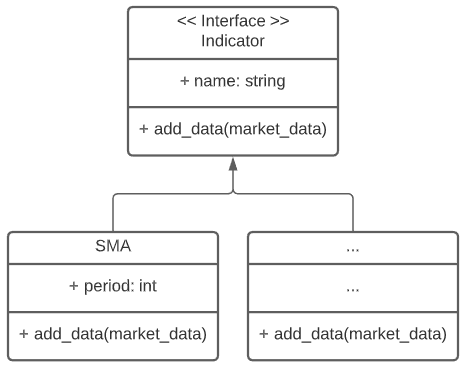
\includegraphics[height=0.34\textheight]{uml/indicators_uml.png}
  \caption{Einfache Darstellung der Indikatoren durch ein Klassendiagramm}
  \label{fig:10}
\end{figure}

Jeder Indikator-Instanz wird ein Name übergeben, welcher durch die Zuweisung an das Attribut \textit{name} der eindeutigen Identifikation eines Indikators dient. Zusätzlich sind alle Indikatoren dazu verpflichtet, eine Methode \textit{add\_data(market\_data)} zu implementieren, welche die indikatorspezifischen Daten an die übergebenen Marktdaten anhängt und zurückgegeben.

%----

\section{Algorithmische Trading Strategien}
\label{sec:algorithmische_trading_strategien}



%----

Auf der Basis der im vorangegangenen Kapitel erstellten Problemanalyse 
und der im Grundlagenkapitel aufgearbeiteten theoretischen Kenntnisse 
wird ein Lösungskonzept erarbeitet.

Bei Software-Projekten entspricht dieses Kapitel typischerweise der 
Analyse \& Design-Phase des \ac{rup}. Typische Ergebnisse dieser Phase sind 
Klassendiagramme etc.

%---------------------------------------------------
\chapter{Implementierung}
\label{cha:implementierung}

In diesem Kapitel wird die konkrete Implementierung des im Kapitel
\ref{cha:loesungskonzept} entwickelten Lösungskonzepts beschrieben.
Hierbei wird auf die konkret verwendeten Entwicklungswerkzeuge etc. 
Bezug genommen.

Bei Software-Projekten besteht dieses Kapitel typischerweise aus den 
Phasen Implementierung \& Test im \ac{rup}.

Zum Beispiel kann man hier auch ein kleines Listing einfügen.

\begin{lstlisting}[language=c,%
                   caption={Überschrift des Quelltexts}]
#include<stdio.h>

int main() {
    // Kommentar
    int answer = 20 << 1;
    answer += 2;
    printf("Hallöchen Welt!\n");
    printf("Die Antwort ist: %d\n", answer);
    return 0;
}
\end{lstlisting}

Manchmal hilft auch eine kleine Tabelle:

\begin{table}[htbp]
\centering
\begin{tabular}{|l|r|}
\hline
\textbf{Messwert a} & \textbf{Messwert b} \\ \hline
9 & 5 \\ \hline
1 & 4 \\ \hline
1 & 3 \\ \hline
\end{tabular}
\caption{Überschrift der Tabelle}
\label{tab:my-table}
\end{table}

Details siehe Tabelle~\ref{tab:my-table}.

%---------------------------------------------------
\chapter{Inbetriebnahme}
\label{cha:inbetriebnahme}

Aufgabe des Kapitels Inbetriebnahme ist es, die Überführung der in 
Kapitel \ref{cha:implementierung} entwickelte Lösung in das betriebliche 
Umfeld aufzuzeigen. Dabei wird beispielsweise die Inbetriebnahme eines 
Programms beschrieben oder die Integration eines erstellten 
Programmodules dargestellt.

Bei der Software-Erstellung entspricht dieses Kapitel der 
Auslieferungsphase (Deployment) im \ac{rup}.

%---------------------------------------------------
\chapter{Evaluierung}

Aufgabe des Kapitels Evaluierung ist es, in wie weit die Ziele der 
Arbeit erreicht wurden. Es sollen also die erreichten Arbeitsergebnisse 
mit den Zielen verglichen werden. Ergebnis der Evaluierung kann auch 
sein, das bestimmte Ziele nicht erreicht werden konnten, wobei die 
Ursachen hierfür auch außerhalb des Verantwortungsbereichs des 
Praktikanten liegen können.

%---------------------------------------------------
\chapter{Zusammenfassung und Ausblick}
\label{cha:zusammenfassung}

\section{Erreichte Ergebnisse}
\label{sec:ergebnisse}

Die Zusammenfassung dient dazu, die wesentlichen Ergebnisse des 
Praktikums und vor allem die entwickelte Problemlösung und den 
erreichten Fortschritt darzustellen. (Sie haben Ihr Ziel erreicht und 
dies nachgewiesen).

\section{Ausblick}
\label{sec:ausblick}

Im Ausblick werden Ideen für die Weiterentwicklung der erstellten Lösung 
aufgezeigt. Der Ausblick sollte daher zeigen, dass die Ergebnisse der 
Arbeit nicht nur für die in der Arbeit identifizierten Problemstellungen 
verwendbar sind, sondern darüber hinaus erweitert sowie auf andere 
Probleme übertragen werden können.

\subsection{Erweiterbarkeit der Ergebnisse}
\label{sub:erweiterbarkeit}

Hier kann man was über die Erweiterbarkeit der Ergebnisse sagen.

\subsection{Übertragbarkeit der Ergebnisse}
\label{sub:uebertragbarkeit}

Und hier etwas über deren Übertragbarkeit.

%-----------------------------------------------------------------------
\appendix

%---
\printbibliography[heading=bibintoc]

%---
\chapter{Anhang A}

%---
\chapter{Anhang B}


\end{document}